\section{Asymptotische Laufzeit}\label{sec:05-asymptotische-laufzeit}

%=====================================================================================================================

\subsection{\texorpdfstring{$\Theta$}{Theta}-Grundregeln}\label{sec:05-theta-grundregeln}
\ZSFindex{Asymptotische Notationen}
\ZSFindex{O-Notation}
\ZSFindex{Theta-Notation}
\ZSFindexsee{Landau-Notation}{Asymptotische Notationen}

\begin{defbox}[Intuitive Bedeutung für MC]
  \begin{factlist}
    \ZSFFact{$f(n) \in O(g(n))$}{Höchstens so schnell wie $g(n)$ ($\le$). $g$ ist eine obere Schranke.}
    \ZSFFact{$f(n) \in \Omega(g(n))$}{Mindestens so schnell wie $g(n)$ ($\ge$). $g$ ist eine untere Schranke.}
    \ZSFFact{$f(n) \in \Theta(g(n))$}{Exakt so schnell wie $g(n)$ ($=$). Beide haben dieselbe Klasse.}
    \ZSFFact{$f(n) \in o(g(n))$}{Echt langsamer als $g(n)$ ($<$).}
    \ZSFFact{$f(n) \in \omega(g(n))$}{Echt schneller als $g(n)$ ($>$).}
  \end{factlist}
\end{defbox}

\begin{contentbox}[Rechenregeln für MC-Aufgaben]
  \begin{factlist}
    \ZSFFact{Dominanz (Summenregel)}{Der am schnellsten wachsende Term gewinnt und bestimmt die Klasse. Langsamere Terme und Konstanten fallen weg. \\
      *Beispiel:* $3n^2 + n \log n + 100 \in \Theta(n^2)$.}
    \ZSFFact{Produktregel}{Klassen werden multipliziert: $O(f(n)) \cdot O(g(n)) = O(f(n) \cdot g(n))$. \\
      *Beispiel:* $n \cdot O(\log n) = O(n \log n)$.}
    \ZSFFact{Transitivität}{Wenn $f \in O(g)$ und $g \in O(h)$, dann ist $f \in O(h)$. (Gilt für alle Klassen).}
    \ZSFFact{Komplementarität}{$f(n) \in O(g(n)) \iff g(n) \in \Omega(f(n))$.}
  \end{factlist}
\end{contentbox}

%=====================================================================================================================

\subsection{Wachstumsordnung}\label{sec:05-wachstumsordnung}
\ZSFindex{Wachstumsordnung}

\begin{formulabox}
  \textbf{Die Master-Sortierliste (von langsam nach schnell)}
  \\[\ZSFspaceXS]
  \( 1 < \log(\log n) < \log n < \sqrt{n} < n < n \log n < n^2 < n^3 < 2^n < 3^n < n! < n^n \)
  \\[\ZSFspaceXS]
  \TableCellNote{Jede noch so kleine Potenz $n^{0.01}$ wächst asymptotisch schneller als jeder Logarithmus $(\log n)^{100}$.}
  \TableCellNote{Jeder Exponent $1.01^n$ wächst asymptotisch schneller als jedes Polynom $n^{1000}$.}
\end{formulabox}

\begin{contentbox}[Grenzwert-Kriterium für MC]
  Um zwei Funktionen $f(n)$ und $g(n)$ für $n \to \infty$ zu vergleichen:
  \begin{ZSFtable}{Y{0.8} Y{0.7} Y{1.5}}
    \toprule
    \ZSFheaderRow \ZSFhead{Grenzwert $\lim \frac{f(n)}{g(n)}$} & \ZSFhead{Bedeutung} & \ZSFhead{Ergebnis} \\
    \midrule
    $0$ & $f$ wächst echt langsamer & \textbf{\boldmath $f(n) \in o(g(n)) \implies f(n) \in O(g(n))$} \\
    $c > 0$ (Konstante) & beide wachsen gleich schnell & \textbf{\boldmath $f(n) \in \Theta(g(n)) \iff g(n) \in \Theta(f(n))$} \\
    $\infty$ & $f$ wächst echt schneller & \textbf{\boldmath $f(n) \in \omega(g(n)) \implies f(n) \in \Omega(g(n))$} \\
    \bottomrule
  \end{ZSFtable}
\end{contentbox}

\begin{statementbox}[Schnell-Checks für Exponenten \& Logarithmen]
  \begin{itemize}[leftmargin=*]
    \item \hl{Faktoren im Exponent ändern die Klasse:} $2^{2n} = 4^n \implies \Theta(4^n) \ne \Theta(2^n)$.
    \item \hl{Summanden im Exponent ändern die Klasse NICHT:} $2^{n+3} = 8 \cdot 2^n \implies \Theta(2^n)$.
    \item \hl{Logarithmus-Basen sind egal:} $\log_2 n \in \Theta(\log_{10} n)$ (Unterschied ist nur ein konstanter Faktor!).
    \item \hl{Exponent-Basen sind extrem wichtig:} $2^n \ne \Theta(3^n)$. Allgemein gilt $a^n < b^n$ für $a < b$.
    \item \hl{Logarithmus im Exponent:} $2^{\log_2 n} = n$. Aber Achtung bei anderer Basis: $2^{\log_3 n} = n^{\log_3 2} \approx n^{0.63}$ (wächst langsamer als $n$!).
  \end{itemize}
\end{statementbox}

%=====================================================================================================================

\subsection{Standardumformungen}\label{sec:05-standardumformungen}
\ZSFindex{Logarithmusgesetze}
\ZSFindex{L'Hopital}

\begin{contentbox}[MC-Tricks zur Termvereinfachung]
  \begin{factlist}
    \ZSFFact{Exponenten-Tausch}{$a^{\log_b c} = c^{\log_b a}$ \quad \hl{Der wichtigste MC-Trick!} Bringt die Variable aus dem Exponenten in die Basis. \\
      *Beispiel:* $3^{\log_2 n} = n^{\log_2 3} \approx n^{1.58}$.}
    \ZSFFact{Logarithmus-Regeln}{$\log(a^k) = k \log a$. \\
      *Beispiel:* $\log(n^5) = 5 \log n \in \Theta(\log n)$.}
    \ZSFFact{Fakultät mit Stirling}{$n! \approx \left(\frac{n}{e}\right)^n \implies \log(n!) \in \Theta(n \log n)$.}
    \ZSFFact{Logarithmus-Summe}{$\log(a \cdot b) = \log a + \log b$.}
    \ZSFFact{Zweierpotenzen im Logarithmus}{$2^{k \log_2 n} = (2^{\log_2 n})^k = n^k$.}
  \end{factlist}
\end{contentbox}

\begin{procedure}[L'Hôpital-Ableitungsregel (falls Grenzwert unklar)]
  \ProcStep{Ableitungen bilden}{Ersetze $n$ durch $x$ und bilde die kontinuierlichen Ableitungen $f'(x)$ und $g'(x)$.}
  \ProcStep{Grenzwert der Ableitung berechnen}{Bestimme $L = \lim_{x\to\infty} \frac{f'(x)}{g'(x)}$.}
  \ProcStep{Übertragen}{Es gilt $\lim_{n\to\infty} \frac{f(n)}{g(n)} = L$. \\
    *Beispiel:* $\lim \frac{\ln n}{n} \to \lim \frac{1/x}{1} = 0 \implies \ln n < n$.}
\end{procedure}

%=====================================================================================================================

\subsection{Häufige Summen}\label{sec:05-haeufige-summen}
\ZSFindex{Summen}

\begin{tablebox}[Summen-Verhalten auf einen Blick]
  \begin{ZSFtable}{Y{0.6} Y{0.7} Y{1.7}}
    \toprule
    \ZSFheaderRow \ZSFhead{Summe} & \ZSFhead{Formel / Näherung} & \ZSFhead{Laufzeit ($\Theta$) \& MC-Intuition} \\
    \midrule
    $\sum_{i=1}^{n} 1$ & $n$ & \textbf{\boldmath $\Theta(n)$} \quad (Konstante Arbeit $n$-mal addieren) \\
    $\sum_{i=1}^{n} i$ & $\frac{n(n+1)}{2}$ & \textbf{\boldmath $\Theta(n^2)$} \quad (Arithmetische Summe, Dreiecksfläche) \\
    $\sum_{i=1}^{n} i^2$ & $\frac{n(n+1)(2n+1)}{6}$ & \textbf{\boldmath $\Theta(n^3)$} \\
    $\sum_{i=1}^{n} i^k$ & $\approx \frac{n^{k+1}}{k+1}$ & \textbf{\boldmath $\Theta(n^{k+1})$} \quad (Integral-Approximation: $\int x^k \in \Theta(x^{k+1})$) \\
    $\sum_{i=0}^{n} q^i \ (q > 1)$ & $\frac{q^{n+1} - 1}{q - 1}$ & \textbf{\boldmath $\Theta(q^n)$} \quad (Geometrisch wachsend: dominiert durch das letzte Glied) \\
    $\sum_{i=0}^{n} q^i \ (q < 1)$ & $\le \frac{1}{1-q}$ & \textbf{\boldmath $\Theta(1)$} \quad (Geometrisch fallend: konvergiert gegen Konstante) \\
    $\sum_{i=1}^{n} \frac{1}{i}$ & $\ln n + \gamma \approx \ln n$ & \textbf{\boldmath $\Theta(\log n)$} \quad (Harmonische Reihe, extrem wichtig für Teiler) \\
    $\sum_{i=1}^{\log n} i$ & $\frac{(\log n)^2 + \log n}{2}$ & \textbf{\boldmath $\Theta((\log n)^2)$} \\
    $\sum_{i=1}^{n} \log i$ & $\log(n!) \approx n \log n$ & \textbf{\boldmath $\Theta(n \log n)$} \\
    $\sum_{i=1}^{n} \sqrt{i}$ & $\approx \frac{2}{3} n^{3/2}$ & \textbf{\boldmath $\Theta(n^{3/2})$} \\
    $\sum_{i=1}^{n} i \log i$ & keine einfache Formel & \textbf{\boldmath $\Theta(n^2 \log n)$} \\
    $\sum_{i=1}^{n} 2^{n-i}$ & $2^n \cdot \sum_{i=1}^{n} 2^{-i} \approx 2^n$ & \textbf{\boldmath $\Theta(2^n)$} \\
    $\sum_{i=1}^{\log n} 2^i$ & $2^{\log n + 1} - 1 = 2n - 1$ & \textbf{\boldmath $\Theta(n)$} \quad (Geometrische Summe bis $\log n$, verdoppelt sich) \\
    $\sum_{i=1}^{n} \frac{n}{i}$ & $n \cdot \sum_{i=1}^{n} \frac{1}{i}$ & \textbf{\boldmath $\Theta(n \log n)$} \quad ($n$ wird aus der Summe ausgeklammert) \\
    \bottomrule
  \end{ZSFtable}
\end{tablebox}

%=====================================================================================================================

\ZSFmanualColumnBreak
\subsection{Schleifen als Summen}\label{sec:05-schleifen-als-summen}
\ZSFindex{Schleifenanalyse}

\begin{procedure}[Kochrezept: Schleifen in Summen übersetzen]
  \ProcStep{Äussere Schleife aufschreiben}{Bestimme die Grenzen der äusseren Schleife (z.B. von $1$ bis $n$) und schreibe diese als Summe: $\sum_{i=1}^n$.}
  \ProcStep{Innere Schleife aufschreiben}{Bestimme die Grenzen der inneren Schleife in Abhängigkeit der äusseren Laufvariable (z.B. von $1$ bis $i^2$) und hänge diese an: $\sum_{i=1}^n \sum_{j=1}^{i^2}$.}
  \ProcStep{Inhalt modellieren}{Ersetze den Rumpf durch $1$ (sofern er $O(1)$ benötigt): $\sum_{i=1}^n \sum_{j=1}^{i^2} 1$.}
  \ProcStep{Nachschlagen \& Auflösen}{Löse die innerste Summe auf und schlage das Ergebnis in der Summen-Tabelle \ZSFsectionref{sec:05-haeufige-summen} nach: \\
    $\sum_{i=1}^n (\text{innere Summe}) = \sum_{i=1}^n i^2 \in \Theta(n^3)$.}
\end{procedure}

%=====================================================================================================================

\subsection{Typische Schleifenmuster}\label{sec:05-typische-schleifenmuster}
\ZSFindex{Schleifenmuster}

\ZSFkeyword*{Platzhalter:} $a(n)$ ist die äussere Grenze, $b(n)$ eine von $i$ unabhängige innere Grenze und $b(i,n)$ eine von $i$ abhängige innere Grenze. $c,p,q$ sind Konstanten.

\subsubsection{Unabhängige und konstante Grenzen}

\begin{loopcatalog}
\LoopPatternTitle{Eine Schleife}
\begin{lstlisting}[style=CodeExpert]
for i in range(a(n)):
    f()
\end{lstlisting}
\LoopPatternResult{a(n)}

\LoopPatternTitle{Unabhängige Grenzen}
\begin{lstlisting}[style=CodeExpert]
for i in range(a(n)):
    for j in range(b(n)):
        f()
\end{lstlisting}
\LoopPatternResult{a(n)\,b(n)}

\LoopPatternTitle{Konstante innere Grenze}
\begin{lstlisting}[style=CodeExpert]
for i in range(a(n)):
    for j in range(c):
        f()
\end{lstlisting}
\LoopPatternResult{a(n)}
\end{loopcatalog}

\subsubsection{Abhängige innere Grenzen}

\begin{loopcatalog}
\LoopPatternTitle{Wachsende innere Grenze}
\begin{lstlisting}[style=CodeExpert]
for i in range(a(n)):
    for j in range(i):
        f()
\end{lstlisting}
\LoopPatternResult{a(n)^2}

\LoopPatternTitle{Schrumpfende innere Grenze}
\begin{lstlisting}[style=CodeExpert]
for i in range(a(n)):
    for j in range(i, a(n)):
        f()
\end{lstlisting}
\LoopPatternResult{a(n)^2}

\LoopPatternTitle{Dreifach gestaffelte Grenzen}
\begin{lstlisting}[style=CodeExpert]
for i in range(a(n)):
    for j in range(i):
        for k in range(j):
            f()
\end{lstlisting}
\LoopPatternResult{a(n)^3}
\end{loopcatalog}

\subsubsection{Multiplikative Updates}

\begin{loopcatalog}
\LoopPatternTitle{Durch Faktor teilen}
\begin{lstlisting}[style=CodeExpert]
i = a(n)
while i > c:
    f()
    i //= q
\end{lstlisting}
\LoopPatternResult{\log a(n)}

\LoopPatternTitle{Mit Faktor multiplizieren}
\begin{lstlisting}[style=CodeExpert]
i = c
while i < a(n):
    f()
    i *= q
\end{lstlisting}
\LoopPatternResult{\log a(n)}

\LoopPatternTitle{Laufvariable potenzieren}
\begin{lstlisting}[style=CodeExpert]
i = c
while i < a(n):
    f()
    i = i ** p
\end{lstlisting}
\LoopPatternResult{\log\log a(n)}
\end{loopcatalog}

\subsubsection{Potenzen in Grenzen und Bedingungen}

\begin{loopcatalog}
\LoopPatternTitle{Potenz in der Abbruchbedingung}
\begin{lstlisting}[style=CodeExpert]
m = 0
while m ** p < a(n):
    f()
    m += 1
\end{lstlisting}
\LoopPatternResult{a(n)^{1/p}}

\LoopPatternTitle{Ausdruck als äussere Grenze}
\begin{lstlisting}[style=CodeExpert]
for i in range(a(n)):
    for j in range(i):
        f()
\end{lstlisting}
\LoopPatternResult{a(n)^2}

\LoopPatternTitle{Potenz als innere Grenze}
\begin{lstlisting}[style=CodeExpert]
for i in range(a(n)):
    for j in range(i ** p):
        f()
\end{lstlisting}
\LoopPatternResult{a(n)^{p+1}}
\end{loopcatalog}

\subsubsection{Zusammengesetzte Grenzen}

\begin{loopcatalog}
\LoopPatternTitle{Teilerprüfung: gesamte Laufzeit}
\begin{lstlisting}[style=CodeExpert]
for i in range(a(n)):
    for j in range(1, i + 1):
        if i % j == 0:
            f()
\end{lstlisting}
\LoopPatternResult{a(n)^2}

\LoopPatternTitle{Summe zweier Laufvariablen}
\begin{lstlisting}[style=CodeExpert]
for i in range(a(n)):
    for j in range(a(n)):
        for k in range(i + j):
            f()
\end{lstlisting}
\LoopPatternResult{a(n)^3}
\end{loopcatalog}

%=====================================================================================================================

\subsection{Rekurrenzen und Master-Theorem}\label{sec:05-rekurrenzen-und-master-theorem}
\ZSFindex{Rekurrenz}
\ZSFindex{Master-Theorem}
\ZSFindex{Ausrollen}

\begin{contentbox}[Das Einmaleins des Master-Theorems]
  Für Rekurrenzen der Form: \quad $T(n) = a \cdot T\!\left(\frac{n}{b}\right) + f(n)$ \quad ($a \ge 1$, $b > 1$)
  \begin{factlist}
    \ZSFFact{$T(n)$}{Gesamtlaufzeit bei Eingabegrösse $n$}
    \ZSFFact{$a$}{Anzahl der rekursiven Teilprobleme (Verzweigungsfaktor, $a \ge 1$)}
    \ZSFFact{$b$}{Faktor, um den die Problemgrösse geteilt wird ($b > 1$)}
    \ZSFFact{$f(n)$}{Kosten für Aufteilung \& Zusammenführung (äussere Arbeit)}
  \end{factlist}
  \ZSFgapXS
  Wir vergleichen die \hl{Arbeit an den Blättern} $n^{\log_b a}$ mit der \hl{äusseren Arbeit} $f(n)$:
\end{contentbox}

\begin{tablebox}[Die drei Hauptfälle]
  \begin{ZSFtable}{Y{0.4} Y{1.0} Y{1.3} Y{1.3}}
    \toprule
    \ZSFheaderRow \ZSFhead{Fall} & \ZSFhead{Bedingung für $f(n)$} & \ZSFhead{Wer gewinnt? (Dominanz)} & \ZSFhead{Laufzeit $T(n)$} \\
    \midrule
    \textbf{1} & $f(n)$ ist polynomiell kleiner & Blätter gewinnen ($n^{\log_b a}$) & \textbf{\boldmath $\Theta(n^{\log_b a})$} \\
    \textbf{2} & $f(n)$ ist gleich gross & Unentschieden (Balance) & \textbf{\boldmath $\Theta(n^{\log_b a} \log n)$} \\
    \textbf{3} & $f(n)$ ist polynomiell grösser & Äussere Arbeit gewinnt ($f(n)$) & \textbf{\boldmath $\Theta(f(n))$} \\
    \bottomrule
  \end{ZSFtable}
  \ZSFgapXS
  \TableCellNote{Hinweis: "`Polynomiell"` bedeutet, der Unterschied muss mindestens Faktor $n^\epsilon$ ($\epsilon > 0$) sein. Ein blosser $\log n$-Faktor reicht nicht für Fall 1 oder 3!}
\end{tablebox}

\begin{procedure}[Kochrezept: Ausrollen für Nicht-Standard-Rekursionen]
  \ProcStep{Einsetzen (Ausrollen)}{Ersetze den rekursiven Term mehrmals durch sich selbst, um das Muster zu erkennen: \\
    $T(n) = T(n-1) + n = T(n-2) + (n-1) + n = T(n-k) + \sum_{i=0}^{k-1} (n - i)$.}
  \ProcStep{Abbruch finden}{Stelle die Abbruchbedingung auf. Meist wenn das Argument $1$ wird: $n - k = 1 \implies k = n - 1$.}
  \ProcStep{Summe aufstellen}{Ersetze $k$ in der Summe und setze die Basis (z.B. $T(1) = c$) ein: \\
    $T(n) = T(1) + \sum_{j=2}^n j = c + \frac{n(n+1)}{2} - 1$.}
  \ProcStep{Klasse ablesen}{Asymptotischen Rumpf ablesen: $T(n) \in \Theta(n^2)$.}
\end{procedure}

\begin{statementbox}[Beliebte MC-Rekursionen auf einen Blick]
  \begin{itemize}[leftmargin=*]
    \item $T(n) = T(n-1) + 1 \implies \Theta(n)$ \quad (Konstante Arbeit auf jeder Stufe)
    \item $T(n) = T(n-1) + n \implies \Theta(n^2)$ \quad (Lineare Arbeit auf jeder Stufe, arithmetische Reihe)
    \item $T(n) = T(n/2) + 1 \implies \Theta(\log n)$ \quad (Binäre Suche)
    \item $T(n) = 2 T(n/2) + n \implies \Theta(n \log n)$ \quad (Merge Sort)
    \item $T(n) = 2 T(n-1) + 1 \implies \Theta(2^n)$ \quad (Fibonacci-artig, exponentieller Baum)
  \end{itemize}
\end{statementbox}

\begin{contentbox}[Rekursionsbaum-Modell]
  \begin{center}
    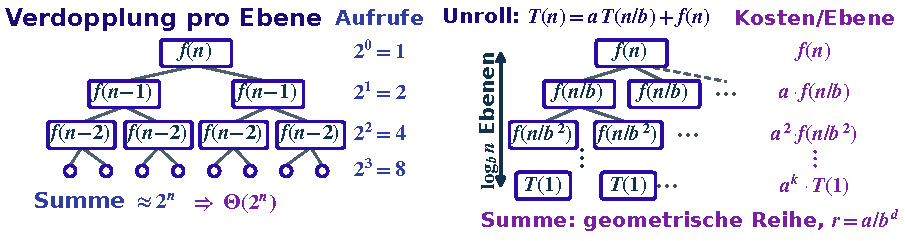
\includegraphics[width=\columnwidth]{Images/asymptotic-recursion-tree-level-costs.pdf}
  \end{center}
\end{contentbox}

\begin{codeboxfirst}[Typische rekursive Implementierungen]
\begin{lstlisting}[style=CodeExpert]
# 1. Zwei rekursive Aufrufe (z.B. Fibonacci)
def fib(n):
    if n <= 1: return n
    return fib(n-1) + fib(n-2)             # -> Theta(phi^n) ~ Theta(1.618^n)
\end{lstlisting}
\end{codeboxfirst}

\begin{codeboxmid}[Viele rekursive Aufrufe]
\begin{lstlisting}[style=CodeExpert]
# 2. n-fache Rekursion (Fakultäts-Aufrufe)
def f(n):
    if n <= 1: return
    for i in range(n):
        f(n-1)                             # -> Theta(n!)
\end{lstlisting}
\end{codeboxmid}

\begin{codeboxlast}[Einfache rekursive Halbierung]
\begin{lstlisting}[style=CodeExpert]
def h(n):
    if n <= 1: return
    h(n // 2)                              # -> Theta(log n)
\end{lstlisting}
\end{codeboxlast}

\begin{contentbox}[Rekursion und Rückgaben]
  \begin{center}
    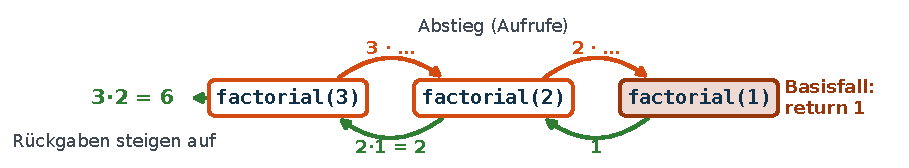
\includegraphics[width=\columnwidth]{Images/recursion-factorial-call-return-trace.pdf}
  \end{center}
\end{contentbox}
